\chapter{Object~Detection}
\label{chap:detection} 


\section{Introduction}


\subsection {Image preparation}

One thing which was noticed in the implementation of the segmentation tool from chapter \ref{chap:bootstrap} was that the original images were often much clearer than the scaled down images for a human annotator to see fine details.

With that in mind I focused on preserving resolution for the annotation process. There may be other reasons to prefer smaller images, such as faster training or inference (which we explore below in section \ref{sec:image_size}, faster loading, reduced memory size, or reduce disk space. 

The additional benefit to preserving resolution is that performance of a given object detector has generally been shown to be better with higher image resolution, when training on data with a limited number of classes, we hypothesis that it is possible to get away with larger image sizes by using much smaller crops of the original images to train, as long as the objects fit in the image crops. We do some experiments on this idea in \ref{sec:crop_size}.

As a counter example the images in the PASCAL VOC \cite{Everingham}, or COCO\cite{Lin2014} datasets have a large range of scales, where many large objects which occupy almost the entirity of the image. For the majority of data experimented on in this thesis, the objects of interest occupy an area much smaller than the whole image size. An analysis of the object sizes in the datasets can be seen in \ref {


\begin{figure}[ht]
\centering
%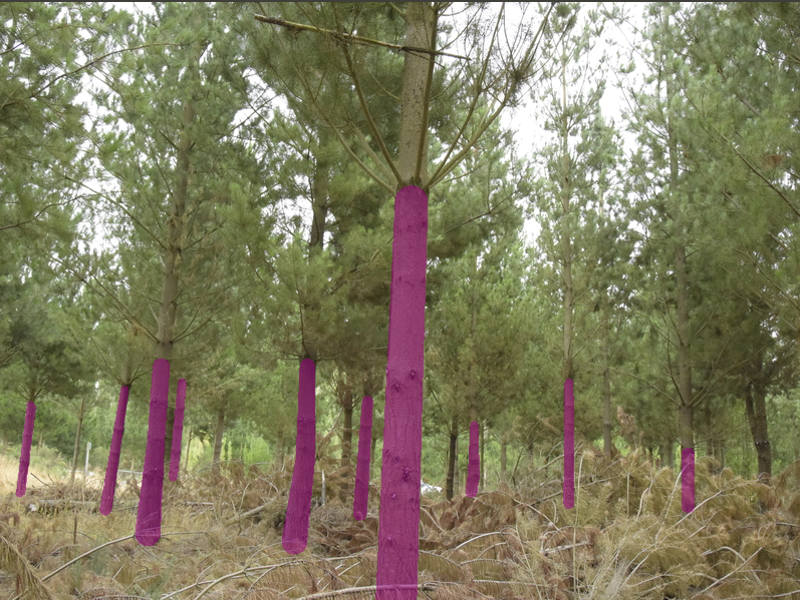
\includegraphics[width=0.9\linewidth]{bootstrap/trees_example.png}

\caption{Object bounding box sizes}
\label{fig:crop_size}
\end{figure}



I also have success in using simpler models as the backbone of the object detection network (for example ResNet--18), which enables larger images in both training and evaluation. Time taken for evaluation and training is also much improved relative to using larger networks. For the smaller datasets in our experiments I did not see large improvements in accuracy when using larger backbone networks.



% We use images of a fixed size in order to train our network (for the purposes of processing images in batches), however because our network is a fully convolutional network we can then test on images of variable size. We show the effect of this processing later, as compared to training with full size images with batches of size one.

% Data augmentation is used to add variety. We use random scales (0.8 to 1.25), crops and rotations (-5 to 5 degrees). We adjust colours on a per colour channel basis ($ \gamma = 0.9 $ to $ \gamma=1.1 $ )  $ x_a = x^{\gamma} $.

% After scaling and rotation, we then crop an area of the image of $440 \times 440$ pixels (the original image size in the trees dataset is $800 \times 600$, down-scaled from the original photos of approximately 25 megapixels.

% We employ image whitening as a last step, subtracting an approximate global mean (r, g, b) $ (0.485. 0.456, 0.406) $ and dividing by standard deviation $ (0.229, 0.224, 0.225) $ as to ensure consistency with the pre-processing used in ImageNet training with the pre--trained model.


\subsection {Object detection}

The object detection method I have been using for the following experiments is a modified RetinaNet \cite{Lin2017} as a strong near-state of the art object detector and having a simple implementation as a single stage object detection method. 






\subsection {Network architecture}
\label{sec:architecture}


Some parameters and network architectures differ from the original paper. For the most part the modifications are small things which seem to enable it to learn better on the kind of small datasets I experiment with below. 

These include adding extra residual layers to the decoder, shown in figure \ref{fig:detection_network}. It is more similar to the network shown in  \ref{chap:bootstrap} than the \gls{FCN} network. A key difference is that the weights between class subnets nor box subnets are shared (the original shares weights between class subnets), as it was found it to slow down initial training considerably. 


Other differences are necessary to accomodate different box sizes (usually using additional finer layer(s) of anchor boxes to handle small objects).

\subsection {Loss function}
\label{sec:loss}


The experiments use a modified version of the Focal Loss \cite{Lin2017} to handle the class imbalance (negative vs. positive) present when sampling anchor box predictions densely.

The basic \gls{CE} equation for prediction $p$ and label $y$ is given:

\begin{equation}
CE(p, y) = x
  \begin{cases}
  \end{cases}
\label{eq:cross_entropy}
\end{equation}



\subsection {Evaluation}
\label{sec:evaluation}



\section{Experiments}
\label{sec:detection_experiments}



\subsection {Single vs. multi class}
\label{sec:multi_class}



\subsection {Crop size}
\label{sec:crop_size}



\section {Effect of scale}
\label{sec:architecture}



\section {Incremental classes}
\label{sec:incremental}


\section {Calibration}
\label{sec:calibration}
